% ==========================================
%          Document class & packages
% ==========================================

\documentclass[12pt]{article}

\usepackage[a4paper,
            left=2.5cm,
            right=2.5cm,
            top=3.5cm,
            bottom=2.5cm]{geometry}

\usepackage{inter}
\renewcommand{\familydefault}{\sfdefault}

\usepackage{fancyhdr}
\usepackage{parskip}
\usepackage{microtype}  
\usepackage{xcolor}
\usepackage{csquotes}
\usepackage[backend=biber,style=ieee]{biblatex}
\addbibresource{referencies.bib}  % Nom del fitxer .bib
\usepackage{xurl}
\usepackage{graphicx}
\usepackage{csvsimple}
\usepackage{booktabs}
\usepackage[catalan]{babel}

\addto\captionscatalan{%
  \renewcommand{\tablename}{Taula}%
  \renewcommand{\figurename}{Figura}%
}

% hyperref last
\usepackage{hyperref}


\urlstyle{same}

\hypersetup{
    colorlinks=true,
    urlcolor=black,
    citecolor=black,
    linkcolor=black
}

% ==========================================
%          Page style configuration
% ==========================================

% ---- Main body style ----
\fancypagestyle{body}{%
  \fancyhf{}
  \fancyfoot[R]{\thepage}
  \fancyhead[R]{\textcolor{gray}{\textit{Projecte SuperSònic}}}
  \renewcommand{\headrulewidth}{0.4pt}
  \setlength{\headheight}{16pt}
  \setlength{\headsep}{26pt}
}

% ---- Title / TOC pages (empty header/footer) ----
\fancypagestyle{emptystyle}{%
  \fancyhf{}
  \renewcommand{\headrulewidth}{0pt}
}

% ---- First page of each section ----
\fancypagestyle{firstpage}{%
  \fancyhf{}
  \fancyfoot[R]{\thepage}
  \renewcommand{\headrulewidth}{0pt}
}

\pagestyle{body}

% ==========================================
%          Custom commands
% ==========================================
\newcommand{\sectionstartlow}{\vspace*{0.25\textheight}}

% ==========================================
%          Document metadata
% ==========================================
\title{Projecte SuperSònic}
\author{Arnau Coronado Nadal}
\date{April 2026}

% ==========================================
%          Document start
% ==========================================
\begin{document}

% ---------------- Title page ----------------
\begin{center}
    \vspace*{3cm}

    {\Huge Projecte SuperSònic}

    \vspace{1cm}
    {\Large Estudi dels cabals a la fabrica d'Euromed}

    \vspace{2cm}
    {\large Arnau Coronado Nadal}

    \vspace{1cm}
    {\normalsize April 2026}
\end{center}

\thispagestyle{emptystyle}
\newpage

% ---------------- TOC ----------------
\thispagestyle{emptystyle}
\renewcommand{\contentsname}{Taula de continguts}
\tableofcontents
\newpage

% ---------------- Body ----------------
\pagenumbering{arabic}

% ===== Section 1 =====
\section{Introducció}

Euromed, S.A. és una empresa industrial amb seu a Mollet del Vallès (Barcelona), especialitzada en el desenvolupament i producció d'extractes botànics per a la indústria farmacèutica, nutracèutica i alimentària.
L'empresa forma part del grup Euromed \cite{Euromed2024}, amb presència internacional i orientació a mercats europeus, americans i asiàtics.

Segons informació corporativa disponible a la seva pàgina web oficial \cite{Euromed2024}, la companyia disposa d'instal·lacions industrials avançades amb processos d'extracció, purificació i assecat, que impliquen l'ús intensiu de fluids tèrmics, aigua de procés i sistemes auxiliars. Aquestes
instal·lacions requereixen un control rigorós dels paràmetres operatius per garantir tant la qualitat del producte com l'eficiència energètica.

Des del punt de vista operatiu, la planta integra múltiples circuits de fluids (aigua calenta, aigua freda, vapor, etc.) que intervenen directament en els processos productius. El control dels cabals en aquests circuits és un factor crític per a l'optimització del consum energètic i la detecció de possibles desviacions operatives.

El projecte en la seva fase inicial estudia els cabals dels circuits d'aigua de torres i vapor.

% ===== Section 2 =====
\section{Objectiu}

En el context actual d'emergència climàtica global, reconeguda per organismes internacionals com el Panell Intergovernamental sobre el Canvi Climàtic \cite{EU2023}, la reducció del consum energètic i de les emissions de gasos amb efecte d'hivernacle s'ha convertit en una prioritat estratègica per al sector industrial.

La indústria representa aproximadament un 25-30\% del consum energètic final a nivell europeu \cite{IPCC2023}, fet que posa de manifest la importància d'implementar mesures d'eficiència energètica basades en dades reals d'operació.

En aquest marc, el present projecte té com a objectiu principal la caracterització dels cabals en diferents punts de la planta d'Euromed, amb la finalitat de:

\begin{itemize}
    \item Quantificar el comportament real dels fluxos de fluids.
    \item Detectar possibles ineficiències o desviacions respecte als valors esperats.
    \item Proporcionar una base de dades fiable per a futures accions d'optimització
          energètica.
\end{itemize}


L'obtenció de dades experimentals és un requisit imprescindible per a la correcta presa de decisions en entorns industrials, specialment en processos amb elevada dependència energètica.

% ===== Section 3 =====
\section{Material i mètode}

Per a la realització de les mesures s'ha utilitzat el cabalímetre ultrasònic portàtil Flexim Fluxus G608 (Emerson), equip específic per a la determinació no invasiva de cabals en conduccions industrials.

Aquest dispositiu opera mitjançant la tecnologia d'ultrasons per temps de trànsit (transit-time), basada en la diferència de temps que experimenten dues senyals ultrasòniques en propagar-se a favor i en contra del flux del fluid. Aquesta diferència temporal ($\Delta t$) és directament proporcional a la velocitat mitjana del fluid, i permet calcular el cabal volumètric amb elevada
precisió \cite{Emerson2024}.

Els sensors s'instal·len externament a la canonada (clamp-on), evitant qualsevol intervenció mecànica sobre el sistema. Aquesta característica presenta avantatges rellevants en entorns industrials:
\begin{itemize}
    \item Eliminació de parades de producció per instal·lació.
    \item Absència de pèrdues de càrrega.
    \item Aplicabilitat a múltiples materials i diàmetres de canonada.
\end{itemize}

Durant el desenvolupament del projecte, el cabalímetre s'ha utilitzat en diferents punts representatius dels circuits de fluids de la planta, seguint criteris d'accessibilitat, rellevància energètica i representativitat del procés. Les mesures s'han realitzat en condicions operatives normals per garantir la validesa dels resultats obtinguts.


\subsection{Aigua de torres (AT)}

Per fer les mesures d'aigua de torres s'ha utilitzat el sensor CDP2NH1.

Cal destacar que, durant la redacció d'aquest informe, s'ha executat una actuació consistent en la instal·lació de vàlvules automàtiques a les plantes E-800 i E-900/E-1000. L'impacte d'aquesta modificació s'analitzarà durant els pròxims mesos a partir de les dades de seguiment.

Els punts de mesura del circuit d'aigua de torres es mostren a la Figura~\ref{fig:punts_at}.

\begin{figure}[htbp]
    \centering
    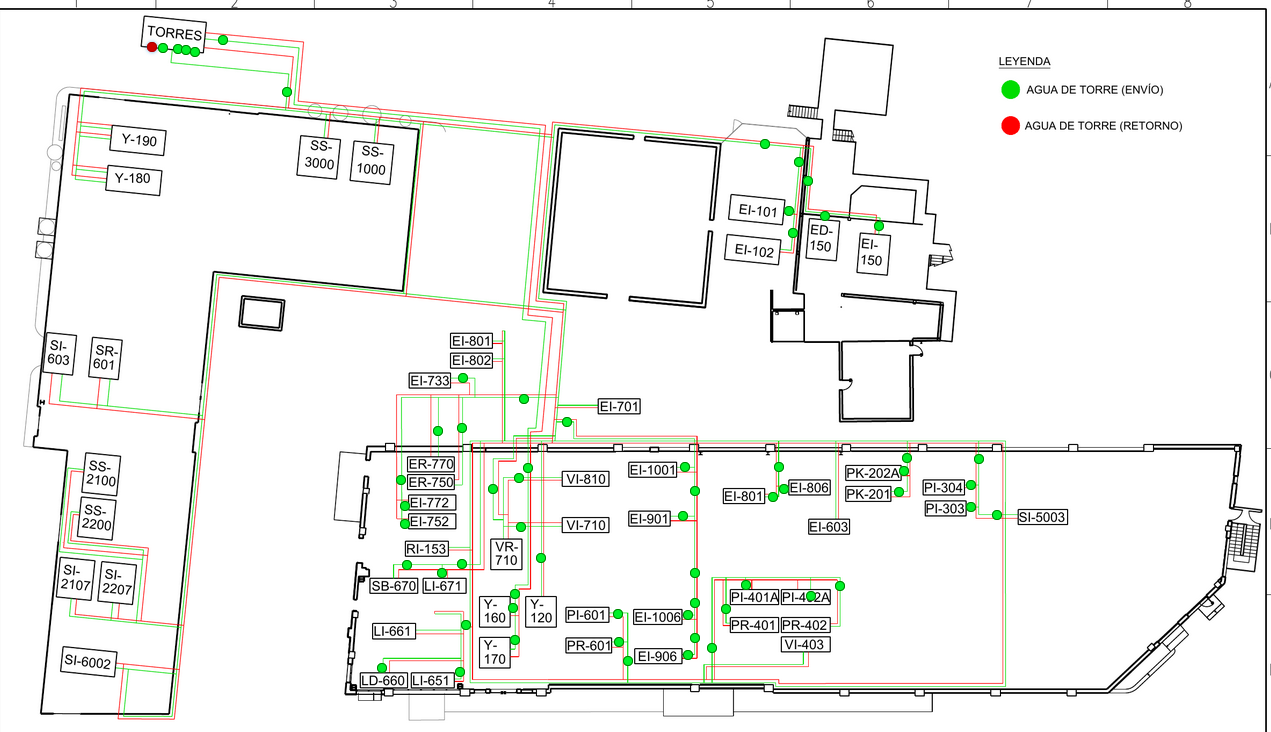
\includegraphics[width=0.85\textwidth]{report_figures/punts_at.png}
    \caption{Punts de mesura del circuit d'aigua de torres (AT).}
    \label{fig:punts_at}
\end{figure}

\subsection{Vapor (STE)}

Per fer les mesures de vapor s'ha fet servir el sensor GRM1SH3.

El circuit de vapor està recobert per un aïllament tèrmic, i per tal de realitzar mesures amb el sensor ultrasònic és necessari aplicar una capa de pintura superficial que evita possibles interferències mecàniques a la canonada. Per aquest motiu, els punts de mesura en el circuit de vapor són més limitats en comparació amb altres serveis del procés. Addicionalment, el consum de vapor presenta una variabilitat significativa en funció de les condicions operatives, fet que requereix campanyes de mesura prolongades (superiors a 24 hores) per obtenir valors representatius.

Els punts de mesura del circuit de vapor es detallen a la Taula~\ref{tab:taula_punts_vapor} i es representen a la Figura~\ref{fig:punts_vapor}.


\begin{table}[htbp]
    \centering

    \caption{Punts de mesura del circuit de vapor}
    \label{tab:taula_punts_vapor}

    \begin{tabular}{lll}
        \toprule
        \textbf{Punt de mesura} & \textbf{Nom inicial} & \textbf{Codi} \\
        \midrule
        E800                    & PM-V-1               & STE-1         \\
        Secadores               & PM-V-2               & STE-2         \\
        PEC                     & PM-V-3               & STE-3         \\
        Nautas                  & PM-V-4               & STE-4         \\
        V800                    & PM-V-5               & STE-5         \\
        V700                    & PM-V-6               & STE-6         \\
        P400                    & PM-V-7               & STE-7         \\
        Atomizador 1a planta    & PM-V-8               & STE-8         \\
        Atomizador 2a planta    & PM-V-9               & STE-9         \\
        S600                    & PM-V-10              & STE-10        \\
        S6000                   & PM-V-11              & STE-11        \\
        \bottomrule
    \end{tabular}

\end{table}


\begin{figure}[htbp]
    \centering
    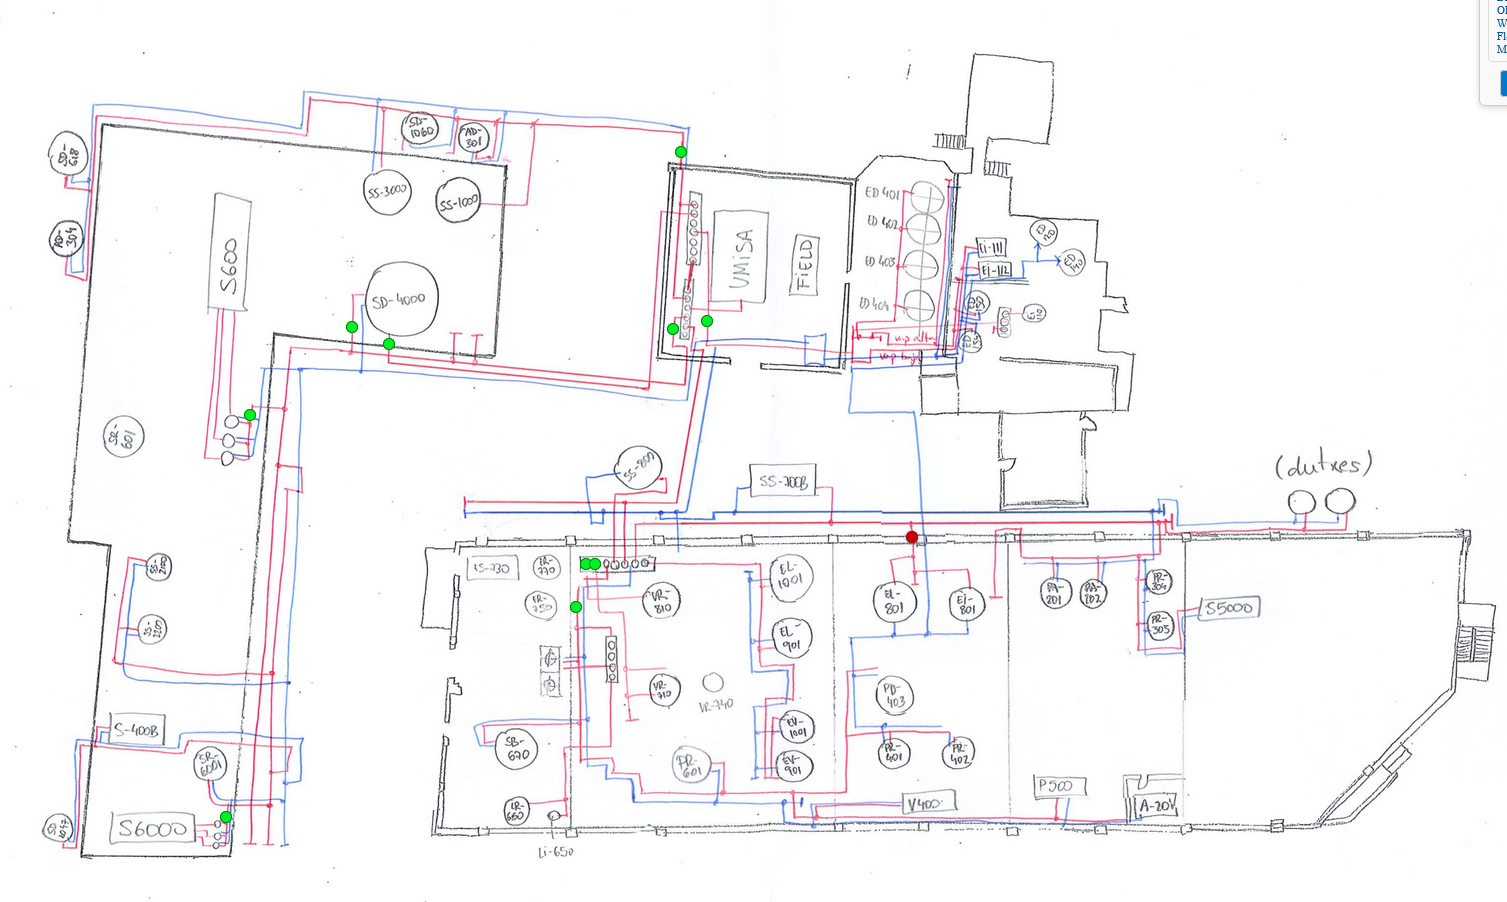
\includegraphics[width=0.85\textwidth]{report_figures/punts_ste.png}
    \caption{Punts de mesura del circuit de vapor.}
    \label{fig:punts_vapor}
\end{figure}



% ===== Section 4 =====
\section{Resultats}

A partir de les mesures realitzades s'han obtingut les següents mesures:


% ===== Section 4 =====
\section{Conclusions}

Ja ho faré jo


% ===== Bibliografia =====
\newpage
\renewcommand{\refname}{Referències}
\printbibliography
\end{document}